\subsection{Setup}

The simulation uses pybullet for physics and few methods from gym-pybullet-drones modified to suit our needs. Important parameters used for experimenting are - number of drones, number of trees and area size. For the most part we've used $3$ drones for exploring a forest area of $900m^2$ with $200$ trees (obstacles) as shown in [picture]. \\

TODO replace with pic
The global planner provides way-points for each drone such that the entire forest is scouted. All way-points are considered as local intermediate goals used to reveal slices of the global occupancy map to the drone, which navigates using a obstacle free path provided by the RRT algorithm. The drone uses a PID controller (code reuse) to follow the desired path.\\

\subsection{Results}

\begin{figure}[h]
\centering
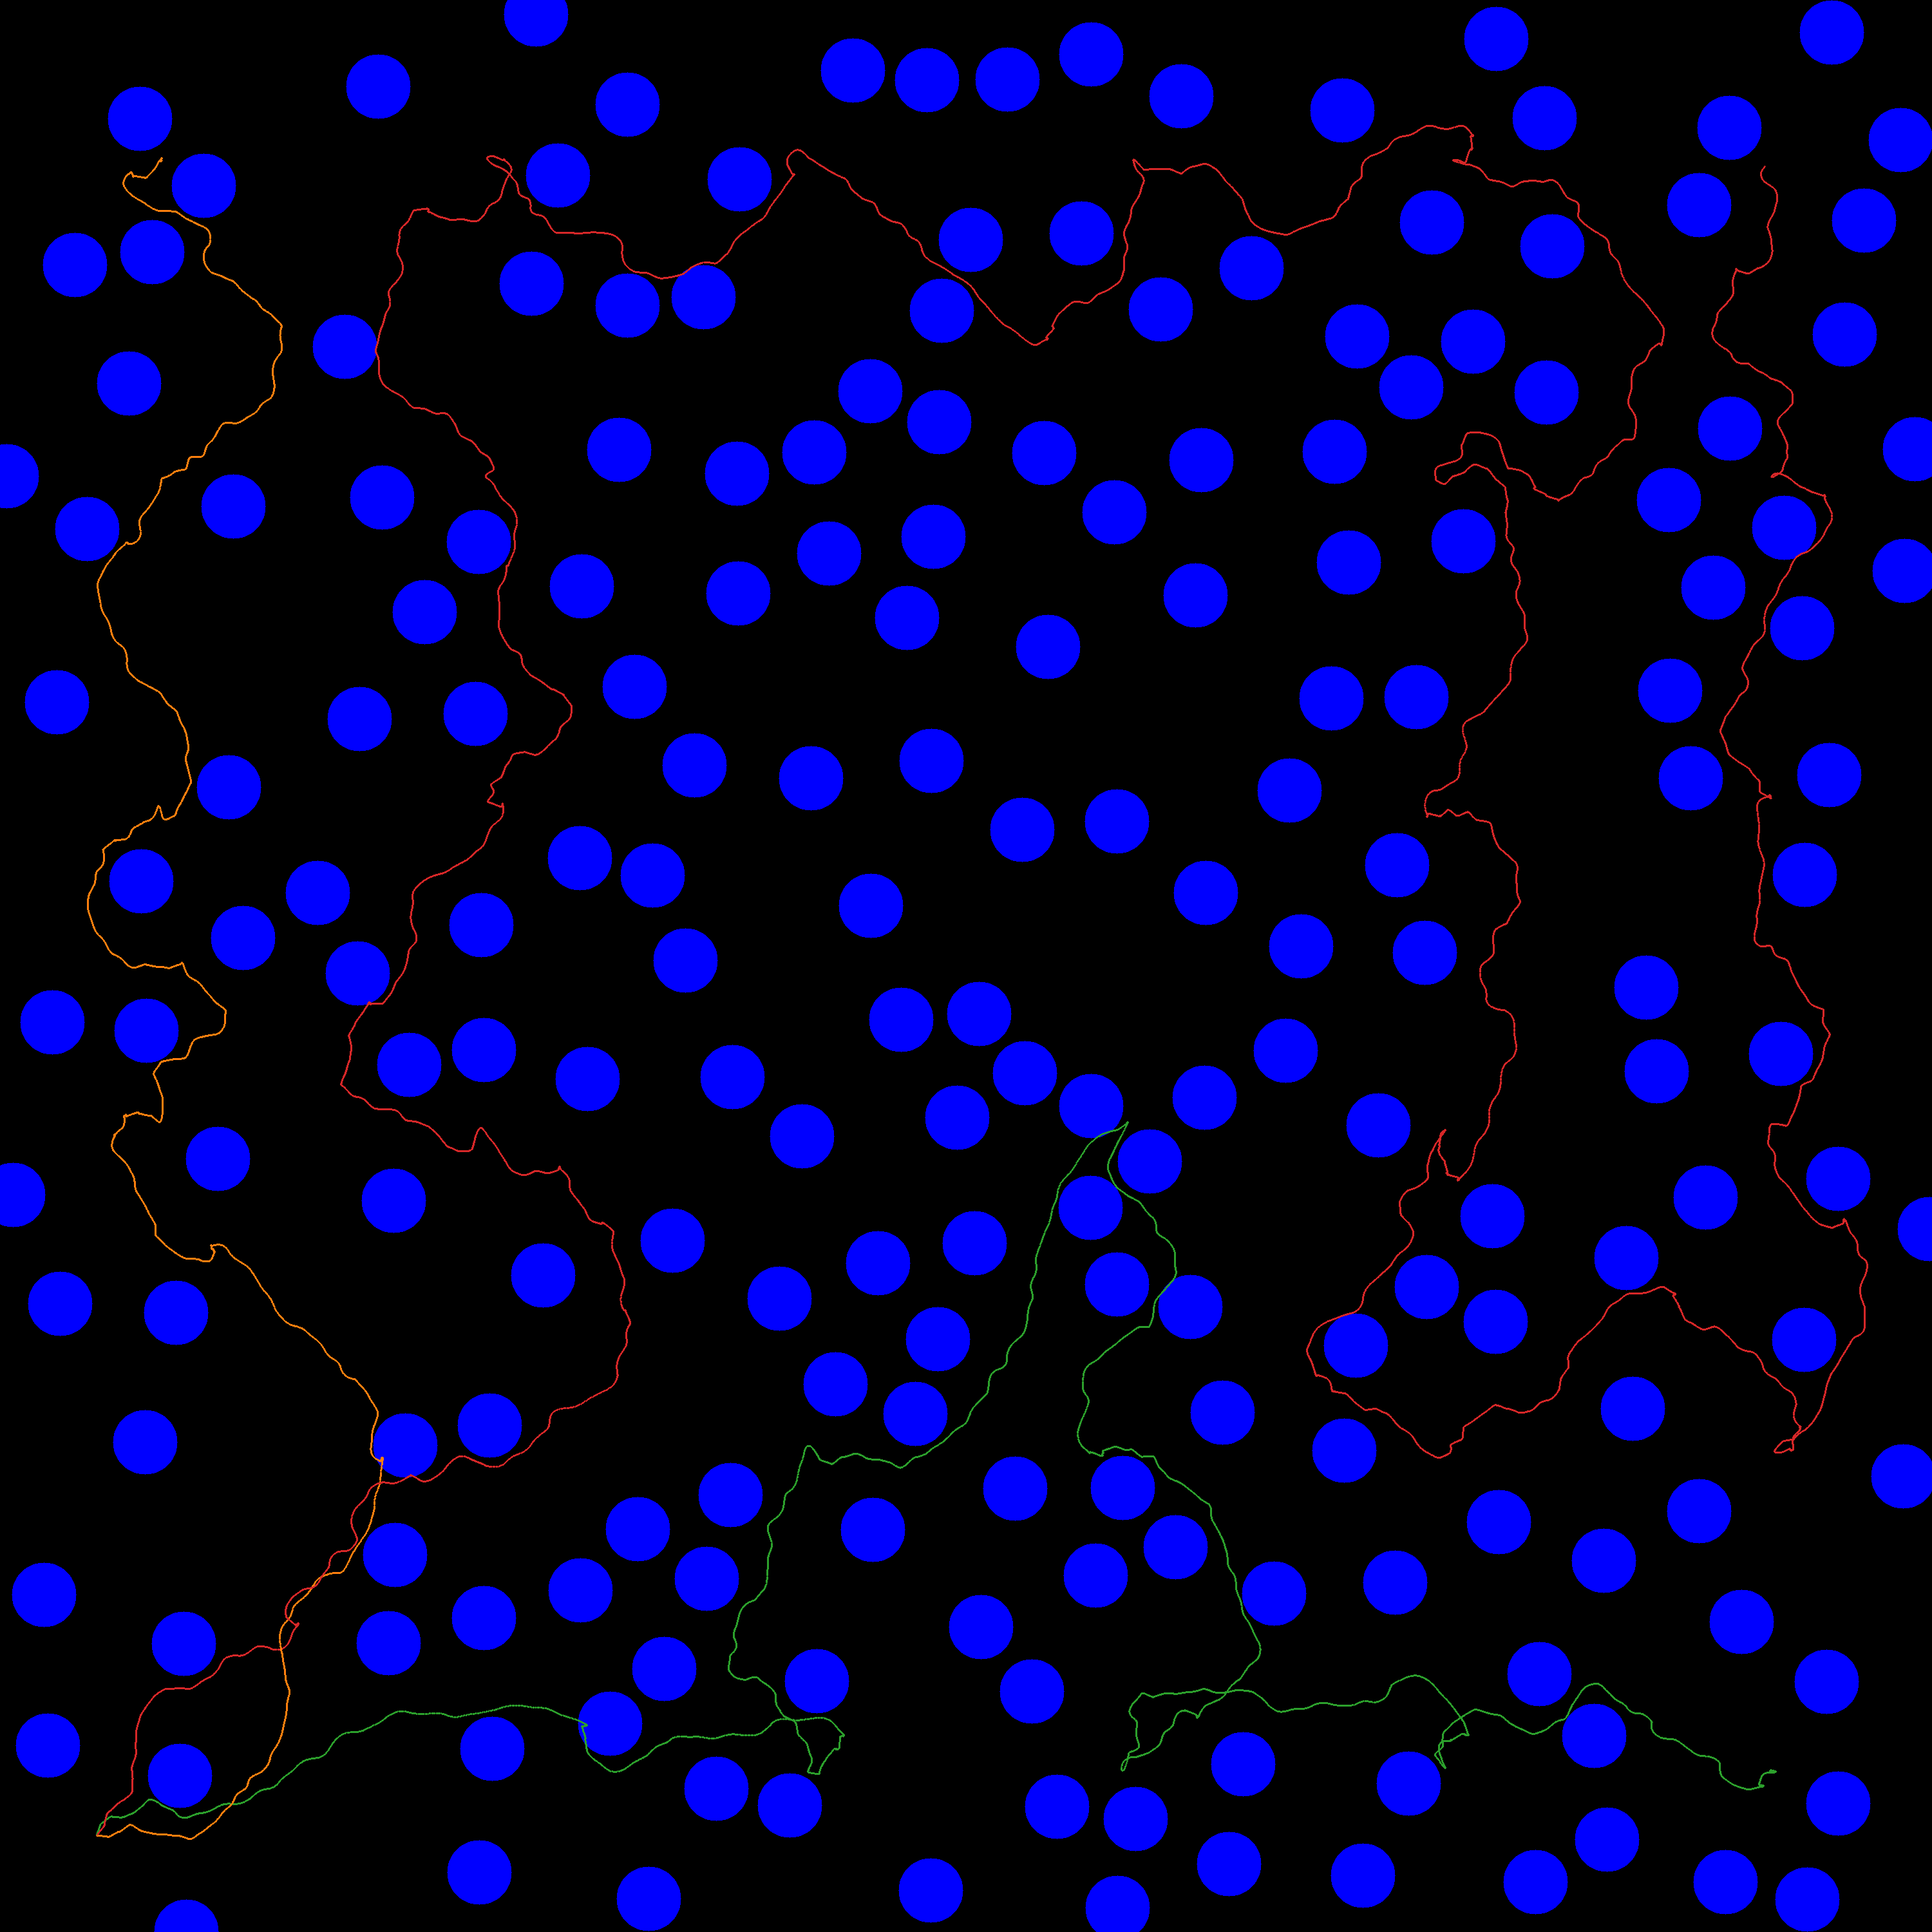
\includegraphics[scale=0.08]{images/preview_map_frame_11193.png}
\caption{Occupancy map on a 30 x 30 m area}
\end{figure}

\begin{figure}[h]
\centering
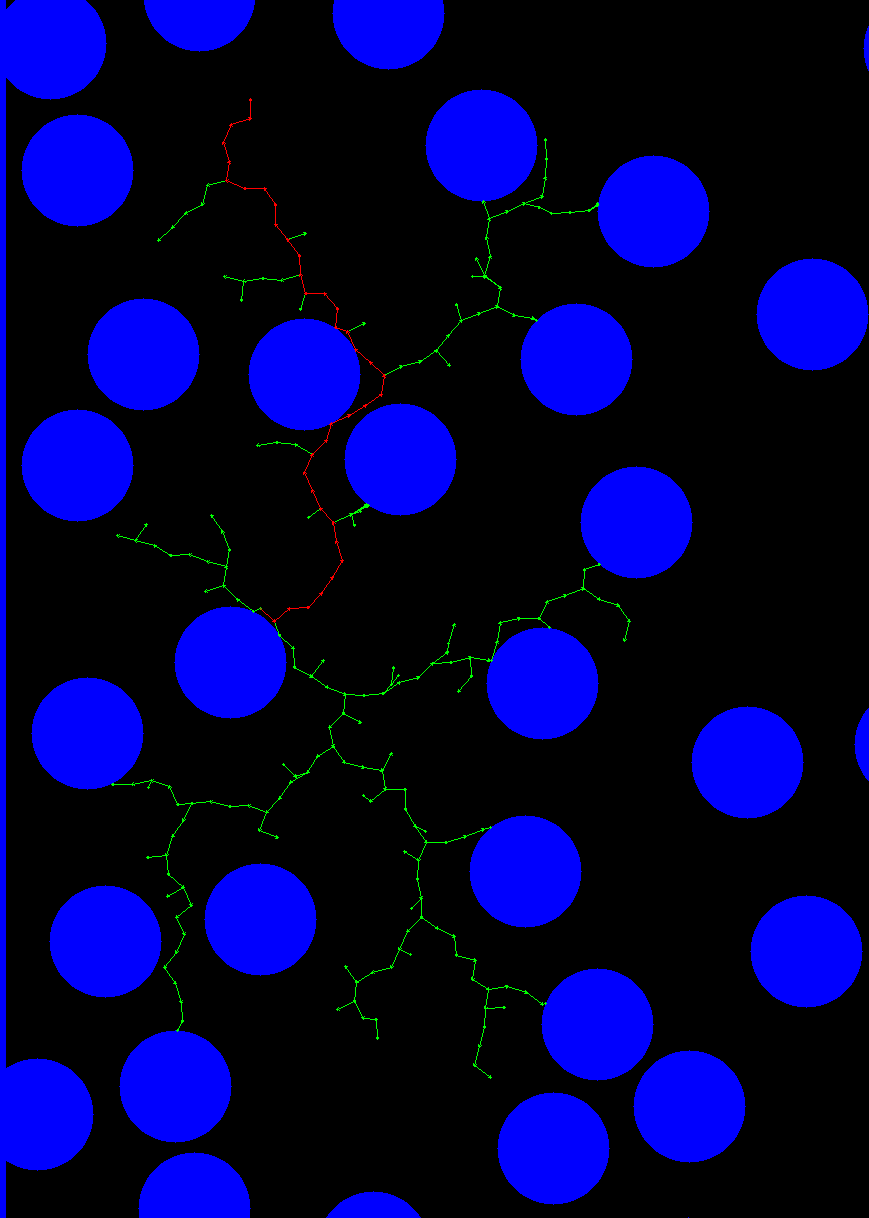
\includegraphics[scale=0.25]{images/rrt_drone_1_iter_6.png}
\caption{RRT on a local occupancy map}
\end{figure}



This \href{https://www.youtube.com/watch?v=JBWNEh0Fis4&ab_channel=ShantnavAgarwal}{video} shows drones navigating in the aforementioned setup.\\

Fig. 1 shows paths (in yellow) followed by each drone to explore the map using paths provided by global path planner and RRT algorithm, which took 8 hours in simulation time (3 mins in practice). \\

[picture] shows the simulation running in a smaller area of $400m^2$ with $100$ trees took x mins. \\

Fig. 2 shows the RRT trees in a local map. As shown the drone doesn't have to know its final goal postion and such a series of local maps can guide the drone towards the goal while offering benefits of faster computation.